\Chapter{Implementáció}

%(6-8 oldal)

% TODO: Ide jöhetnek maguk a kódok
% Meg kell indokolni, hogy miért pont a felhasznált technológiákra esett a választás
% Ebbe a fejezetbe kerülhetnek majd a kódpéldák. Az elejébe annyira nem kellene majd.
% A játékállapot kezelésének konkrét implementációja

\Section{Felhasznált technológiák}

\SubSection{MySQL}
A MySql az egyik legnépszerűbb nyílt forráskódú adatbázis kezelő rendszer, amelyet az Oracle Corporation fejlesztett és támogat. Relációs adatbázisokkal dolgozik, tehát egy nagy adathalmaz helyett az adatokat táblákban tárolja az adatokkal, a táblázat szerkezetekkel, a táblák kapcsolataival, és referencia kulcsaival együtt. Gyors, megbízható, skálázható, és könnyen tanulható. \cite{mysql} 

\SubSection{Java EE}
A Java a Sun által kifejlesztett programozási nyelv és futtatóplatform. A Java nyelv alapjaiban a C++-ra hasonlít, de azzal szemben magas szintű fejlesztést tesz lehetővé. Natív módon támogatja a többszálú programozást és objektum-orientált megoldásai is jóval túlmutatnak a korábbi nyelvekén.

A Java futtatóplatform alapját a Java bájtkód értelmezésére képes JVM képezi, amely gyakorlatilag minden elterjedt operációs rendszerre elérhető. \cite{javaee}

A Java Platform, Enterprise Edition, röviden Java EE, több programkönyvtárat tartalmaz és támogatja a többrétegű, elosztott alkalmazások készítését.

\SubSection{Spring}
A Spring Framework egy moduláris Java keretrendszer, amit azzal a szándékkal alkottak meg, hogy a Java EE alkalmazások programozását könnyebbé tegyék. Néhány előnye:
\begin{itemize}
	\item Könnyű súlyú, kevéssé invazív fejlesztés a régi jó Java objektumokkal (POJO - plain old Java object).
	\item Egyszerűbb teszt írás és kód újra felhasználhatóság.
	\item Loose coupling. Laza kapcsolódást jelent, ami a komponensek függetlenségére utal.
	\item Függőségek egyszerűbb hozzáadása a komponensekhez. (Dependency Injection).
	\item Ismétlődő, redundáns kódrészek (boilerplate kódok) redukálása.
	\item Tranzakció kezelés segítése. \cite{spring}
\end{itemize}

\SubSection{Hibernate}
A Hibernate egy Spring által támogatott ORM technikát megvalósító program könyvtár. Az adatbázisból való lekérésekhez, és az adatbázisban való módosításhoz az objektumainkat tábla oszlopokká kell alakítanunk, lekéréskor pedig fordítva, tábla oszlopainkat kell objektummá alakítani. Ezt hívják ORM-nek (Object Relation Mapping). A Hibernate ezen felül összeállítja SQL parancsainkat, lekérdezéseinket, és kezeli a kapcsolatkiépítést az adatbázissal. Jelentősen csökkenti az adatkezeléshez szükséges kód mennyiségét. \cite{spring}

\SubSection{Maven}
Az Apache Maven (röviden csak Maven) egy projekt kezelő és értelmező eszkösz, amely a project object model (POM) koncepciójára épül. A Maven irányítja a projekt buildelését, fordítását megfelelő formátumra, a függőségek importálását, tehát a projekt felépítését futtatható alkalmazássá. \cite{maven}

\SubSection{TomCat}
Az Apache Tomcat szoftver egy alkalmazás szerver, amely a Java Servlet, JavaServer Pages, Java Expression Language és Java WebSocket egy nyílt forráskódú implementációja. \cite{tomcat}

\SubSection{HTML, CSS, JavaScript}
Minden mai weboldal a HTML, a CSS, és a JavaScript. A HTML az oldal szerkezetét írja le, a CSS a megjelenését, a JavaScript pedig a viselkedést.

\SubSection{AngularJs}
Az AngularJS egy Google által fejlesztett, nyílt forráskódú JavaScript keretrendszer dinamikus webes alkalmazásokhoz. Segítségével nagyban egyszerűsödik a webes alkalmazások frontend fejlesztése és az alkalmazások komponensei egyértelműen elkülönülnek, és rengeteg felesleges boilerplate kód elhagyható. \cite{angularjs}

\SubSection{Git}
A git egy ingyenes és nyílt forráskódú, elosztott verzió kezelő rendszer, amit arra terveztek, hogy a legkisebbtől a legnagyobb projektekig mindent gyorsan és hatékonyan kezeljen. \cite{git}

\Section{JSON Web Token}

Korábban volt szó a token alapú azonosítás előnyeiről. Alkalmazásomban erre a célra JSON Web Tokent használtam (röviden JWT), amely egy nyílt szabvány, ami egy kompakt, önleíró, és önvalidáló eszköz, amellyel biztonságosan, JSON objektumként lehet adatot továbbítani két fél között. Megbízható módszer, mivel digitálisan "alá van írva".

A JSON Web Tokenek 3 fő részből állnak, melyeket ponttal választanak el egymástól: Header (fejléc), Payload (rakomány), Signature (aláírás).

A header tipikusan két információt tartalmaz: a token típusát, ami JWT, és az alkalmazott titkosító algoritmust.
A payload második rész, ami egy entitásról (jellemzően a felhasználóról) tartalmaz információkat. Ebben a részben megadhatunk lejárati időt is.
Signature: Hogy ezt létrehozzuk, először szükségünk lesz a Base64Url kódolású headerre, szintén így kódolt payloadra, egy secretre (egy karakterlánc, amit csak a kibocsátó ismer). Majd ezeket titkosítjuk: az algoritmus egyik paramétereként megadjuk a headert és a payloadot ponttal elválasztva, másik paramétereként a secretet.

A signature-nek fontos szerepe van, ugyanis visszafejtéskor ennek a segítségével megállapíthatjuk, hogy a tartalmat valóban nem módosították, és hogy a küldő valóban az, akinek mondja magát. Ha visszafejtük a teljes tokent, megkapjuk a header.payload kódot és a signature-t. Ha visszafejtjük a signature-t is, szintén megkapjuk a header.payload kódot. Ha a két kód megegyezik, az üzenet érintetlen, hiszen a tokent már egyetlen elírt karakter is érvénytelenítheti.

A tokenből továbbá visszakaphatjuk a payloadban található adatokat is, innen kiolvashatjuk, hogy ki a felhasználó, aki küldte.

Az \ref{fig:jwt} ábra jobb oldalán láthatjuk egy token tartalmát részekre bontva, bal oldat pedig az ezekből az adatokból generált tokent.

\begin{figure}[!h]
	\centering
	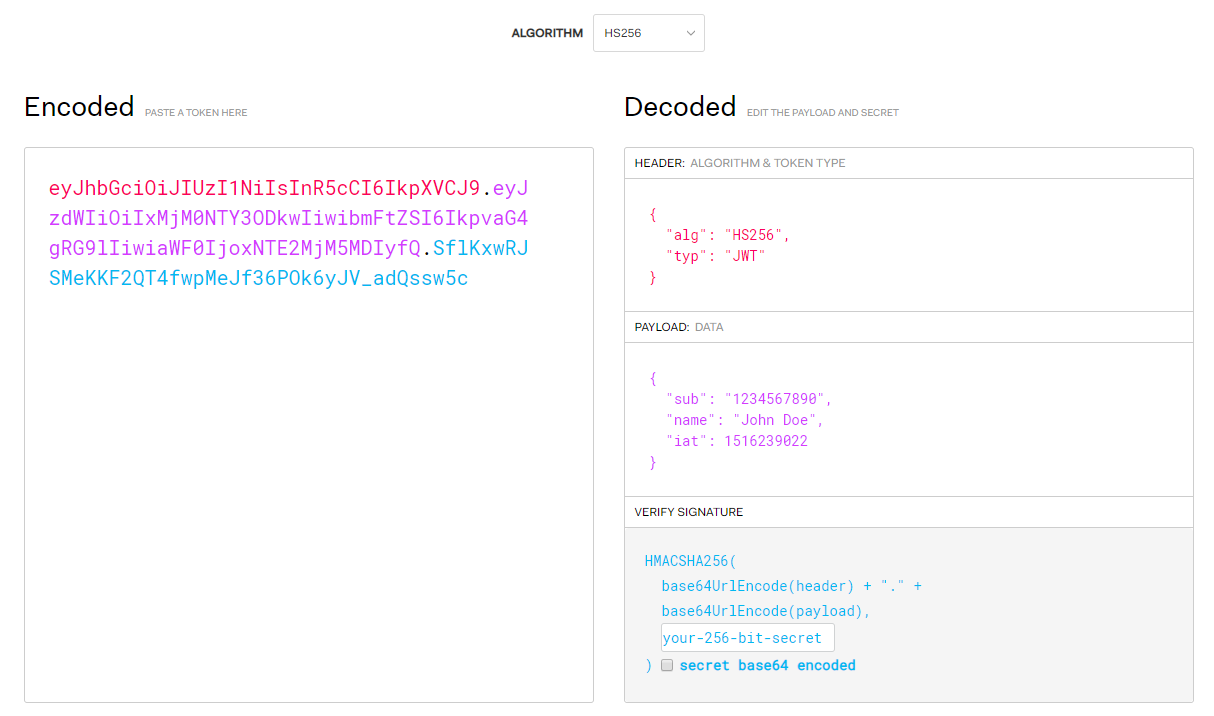
\includegraphics[width=0.95\linewidth]{kepek/jwt.png}
	\caption{\textit{Egy JSON Web Token felépítése}}
	\label{fig:jwt}
\end{figure}

A token fő szerepe az alkalmazásban az azonosítás, és ezáltal a jogosultságok ellenőrzése. A tokent a felhasználó bejelentkezéskor kapja meg, majd minden kérés során elküldi a headerben. Így visszafejtés után a szerver azonosítani tudja a felhasználót, és ellenőrizni tudja a jogosultságát. Ezekre az ellenőrzésekre szükség lehet például, amikor a felhasználó az alkalmazás egy másik oldalára lép, vagy ha a játék során beérkezik egy lépés. A JavaScript futása manipulálható, ezért a szervernek fokozottan kell ellenőrizni a küldő kilétét.

\Section{Backend}


\Section{Frontend}

\SubSection{Nyerés ellenőrzés}

Minden érvényes karakter lerakás után ellenőrizni kell, hogy a játékos nem nyert -e. Ennek implementációját mutatja a \ref{lst:fiveinarow-checkwin} ábra.

\lstinputlisting[caption={\textit{/match/checkstart kérés és válasz minta}}, label={lst:fiveinarow-checkwin}]{kodok/javascript/fiveinarow-checkwin.js}


















